\documentclass[12pt]{article}

\usepackage[T1]{fontenc}
\usepackage[utf8]{inputenc}
\usepackage[icelandic]{babel}
\usepackage{setspace}
\usepackage{comment}
\usepackage{wrapfig}
\usepackage{listings}
\usepackage{courier}
\usepackage{verbatim}
\usepackage{tikz}
\usepackage{caption}
\usepackage{gensymb}
\usepackage{hyperref}
\usepackage{gensymb}


\usepackage{xcolor}
\definecolor{commentgreen}{RGB}{2,112,10}
\definecolor{eminence}{RGB}{108,48,130}
\definecolor{weborange}{RGB}{255,165,0}
\definecolor{frenchplum}{RGB}{129,20,83}

%\usepackage{minted}

\lstdefinestyle{customc}{
  belowcaptionskip=1\baselineskip,
  breaklines=true,
  frame=L,
  xleftmargin=\parindent,
  language=C,
  showstringspaces=false,
  basicstyle=\footnotesize\ttfamily,
  keywordstyle=\bfseries\color{green!40!black},
  commentstyle=\itshape\color{purple!40!black},
  identifierstyle=\color{blue},
  stringstyle=\color{orange},
}

\lstdefinestyle{customasm}{
  belowcaptionskip=1\baselineskip,
  frame=L,
  xleftmargin=\parindent,
  language=[x86masm]Assembler,
  basicstyle=\footnotesize\ttfamily,
  commentstyle=\itshape\color{purple!40!black},
}

\lstset{style=customc,captionpos=t}



\captionsetup{labelformat=empty}

\usepackage{amsmath,amssymb,graphicx,color,enumerate,here}
\setlength{\parindent}{0cm}\newcommand{\Z}{\mathbb{Z}}\newcommand{\R}{\mathbb{R}}\newcommand{\C}{\mathbb{C}}
\newcommand{\N}{\mathbb{N}}\newcommand{\f}[2]{\frac{#1}{#2}}\newcommand{\1}[1]{\frac{1}{#1}}

\voffset=-1.0in
\hoffset=-0.3in
\textwidth=6in
\textheight=9in

\begin{document}
\noindent \large \textbf{Verkefni 3 \hfill Jónas G. Sigurðsson\\
\noindent Tölvugrafík \hfill 
\normalsize  \hfill Mars 2019}\\\\
\begin{small}

\begin{spacing}{2}
\end{spacing}
Þriðja stóra verkefnið í Tölvugrafík var að útfæra tölvuleikinn Tetris í þrívídd. Í stað kubba sem samanstanda af fjórum teningum, þá átti að nota kubba sem samanstanda af þrem teningum.
\begin{spacing}{2}
\end{spacing}
Leiksvæðið átti að vera $6\times 6$ einingar í grunnfleti og 20 einingar að hæð. Einnig átti hver kubbur að detta niður um eina hæð í einu.
\begin{center}
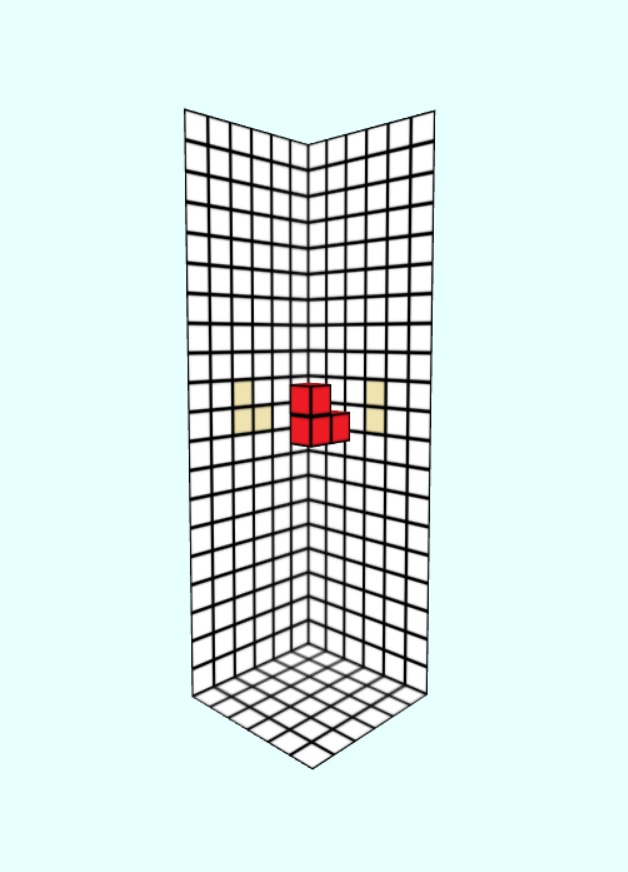
\includegraphics[scale=0.4]{m1}
\end{center}
Hægt er að færa kubbinn sem er að falla til í láréttu plani með örvarhnöppum, snúa um $x$-ás með a/z, $y$-ás með s/x og $z$-ás með $d/c$. Einnig er hægt að láta kubbinn falla hraðar með bilstöng og sleppa honum alveg niður með ENTER.
\begin{center}
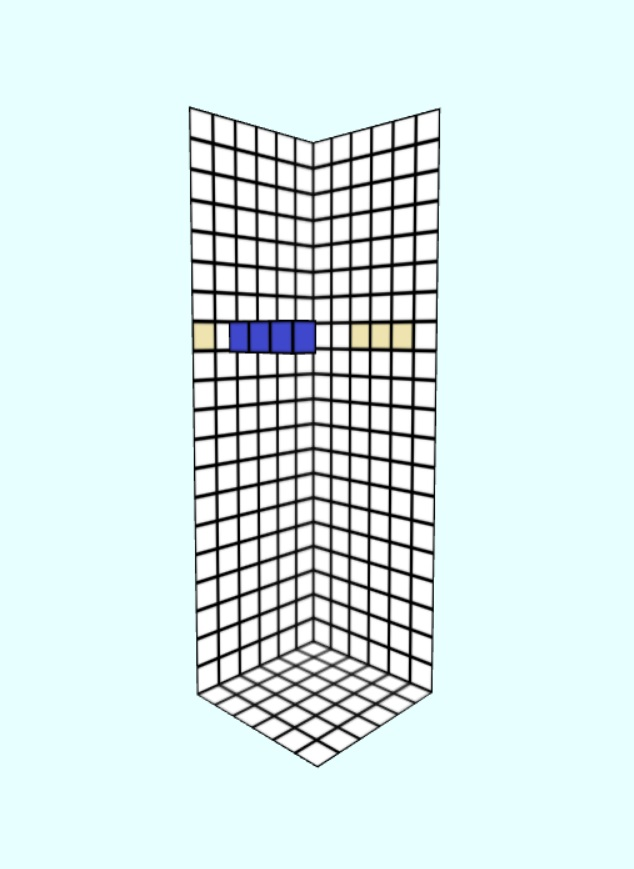
\includegraphics[scale=0.4]{m2}
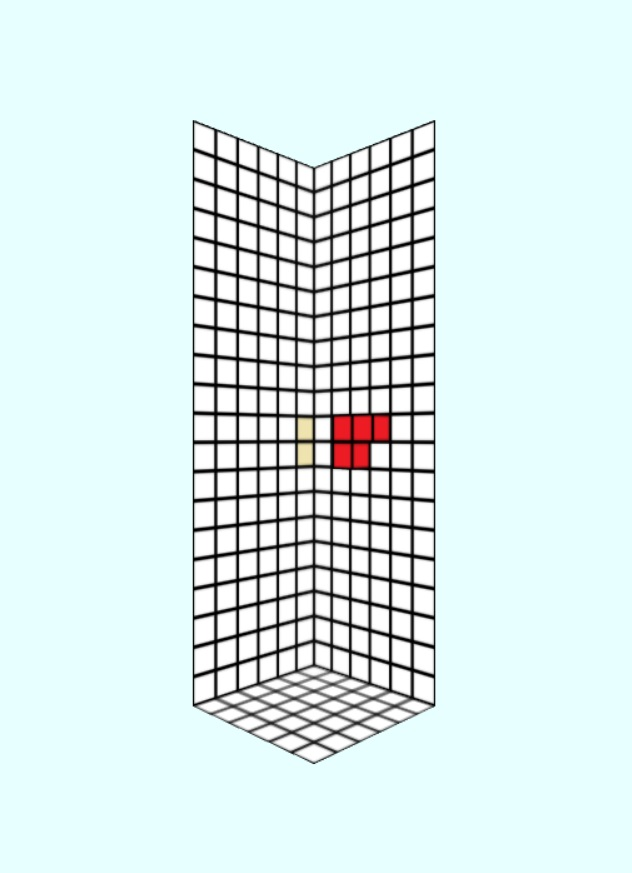
\includegraphics[scale=0.4]{m3}
\end{center}
Er notandi vill fá annað sjónarhorn á leikinn, þá er hægt að snúa leiksvæðinu með músinni og þysja inn og út með því að skruna.
\begin{center}
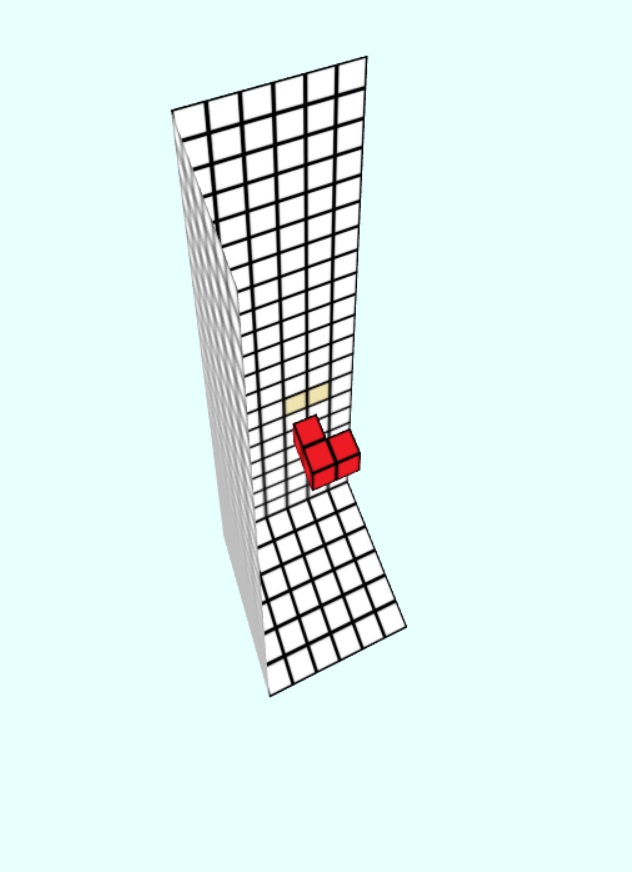
\includegraphics[scale=0.4]{m4}
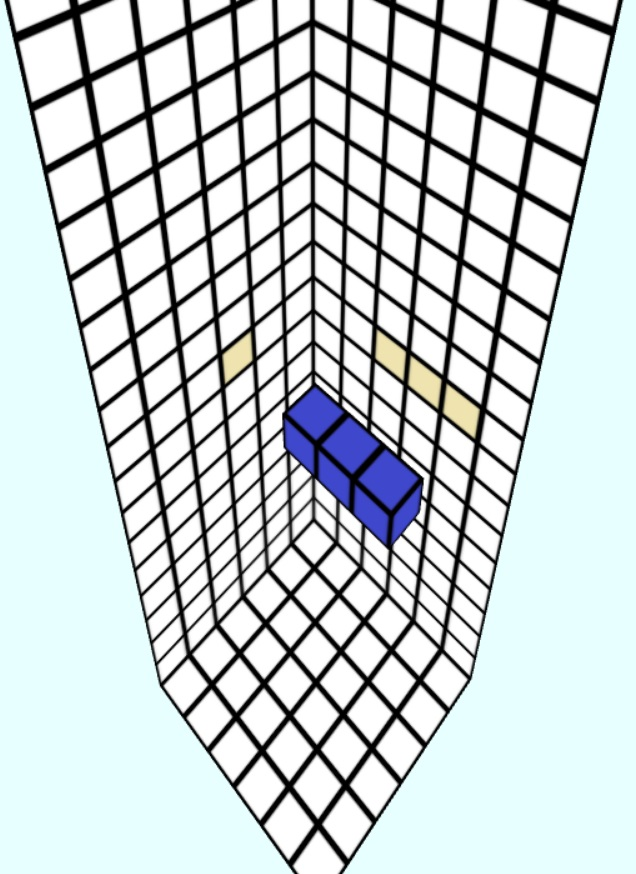
\includegraphics[scale=0.4]{m5}
\end{center}
Kubbarnir staflast rétt og ef að heil hæð fyllist, þá eyðist hún út
\begin{center}
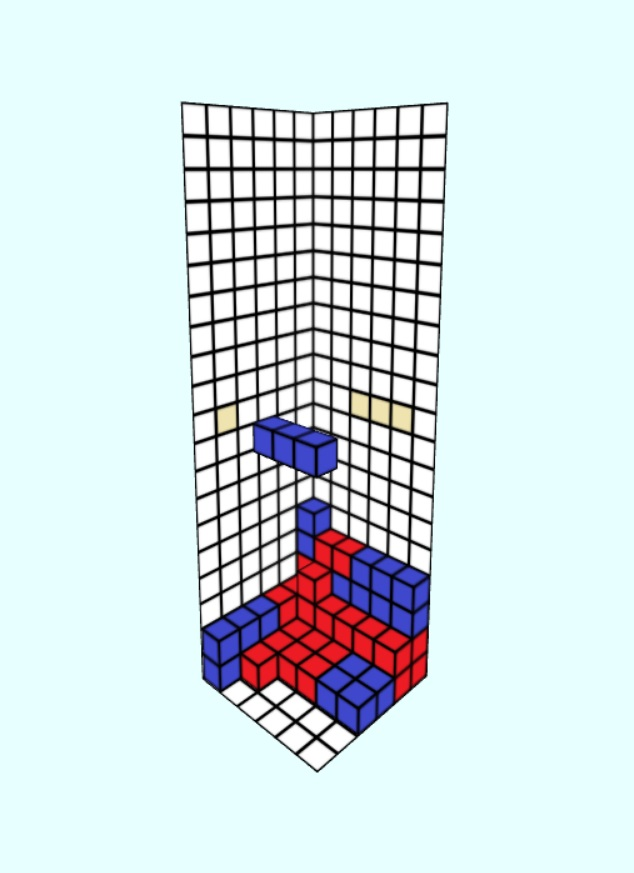
\includegraphics[scale=0.4]{m6}
\end{center}
Aðrir eiginleikar leiksins eru: Skuggar á veggjum sem sýna hvar í loftinu kubburinn er staddur, Leikreglur í bláu boxi vinstra megin við leikinn, stigatafla í rauðu boxi hægra megin við leikinn, teljari sem sýnir hversu mörgum hæðum hefur verið eytt og teljari sem sýnir á hvaða hraða leikurinn er. Hraði leiksins eykst um 1 fyrir hverjar fjórar hæðir sem er eytt og hann fer hraðast upp í 10. Stigagjöfin er eftirfarandi: 150 stig fyrir hvern kubb sem lendir, 500 stig ef kubbnum er sleppt með ENTER og 10.000 stig fyrir að eyða hæð.
\begin{center}
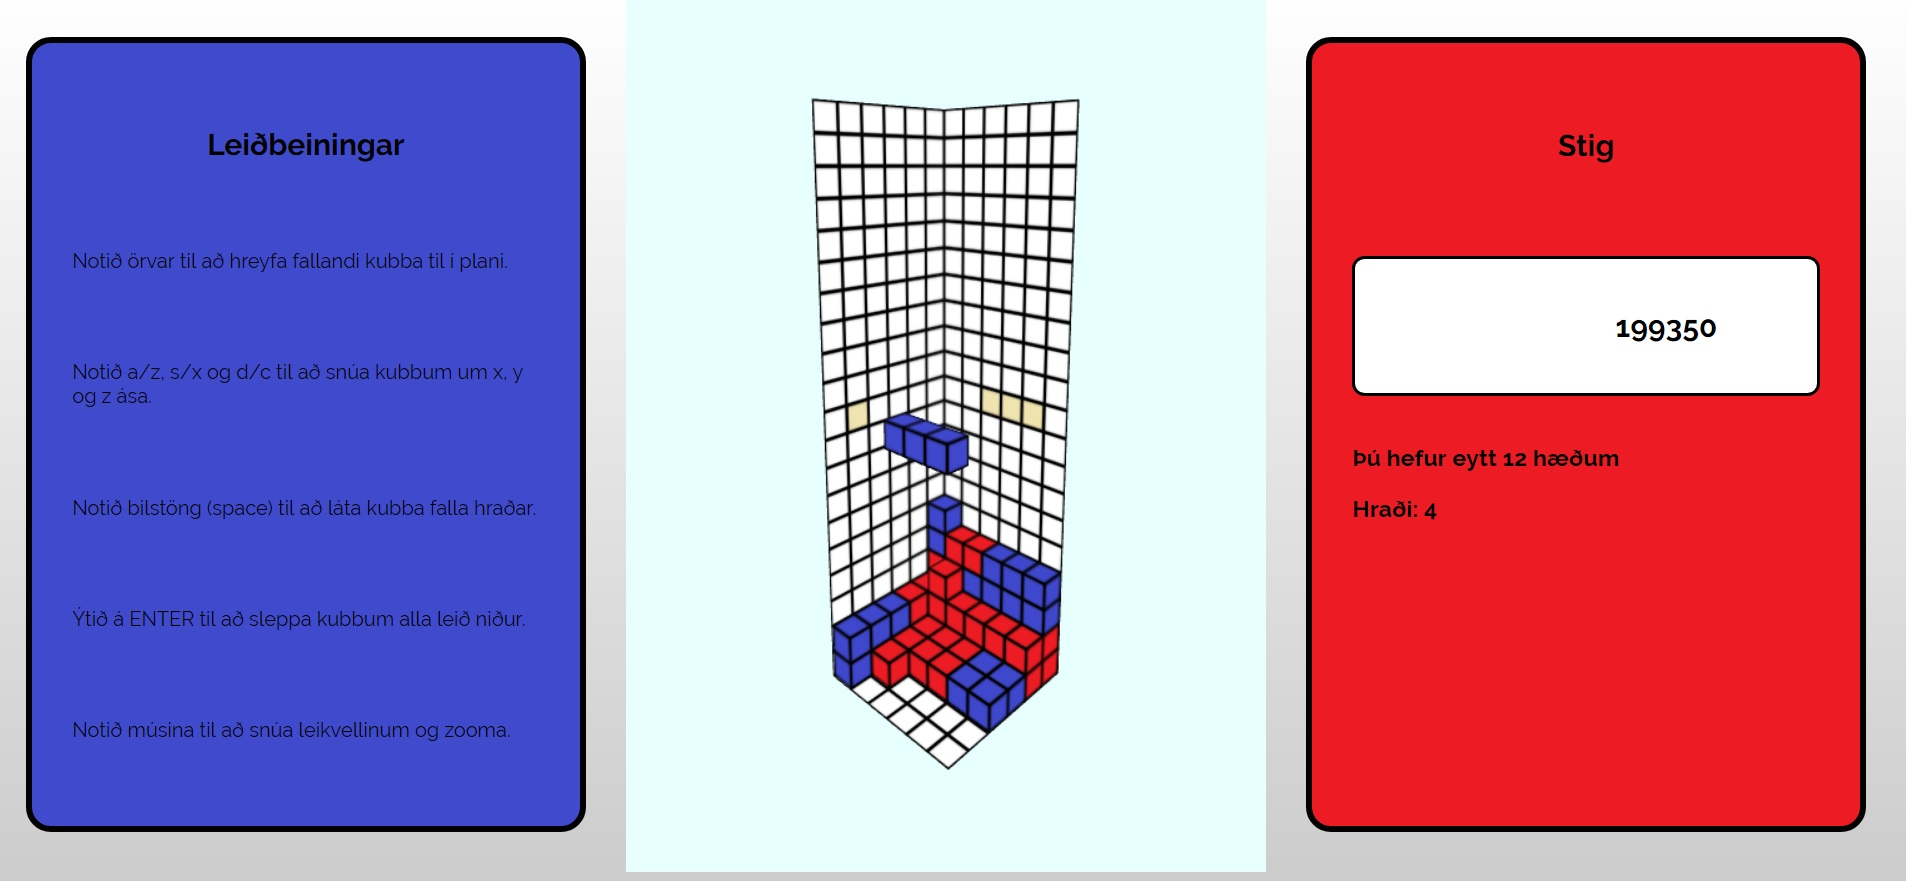
\includegraphics[scale=0.4]{m7}
\end{center}
Ef að kubbarnir staflast alveg upp í topp þannig að nýr kubbur kemst ekki inn á leikvöllinn, þá þurkast allir kubbarnir út og leikurinn býður eftir að notandinn ýti á G til að hefja nýjan leik. Á meðan beðið er sér notandinn hversu mörg stig hann vann sér inn, hversu mörgum hæðum hann eyddi og hraðann sem kubbarnir voru komnir á. Öll tölfræðin núllast út um leið og ýtt er á G.
\begin{center}
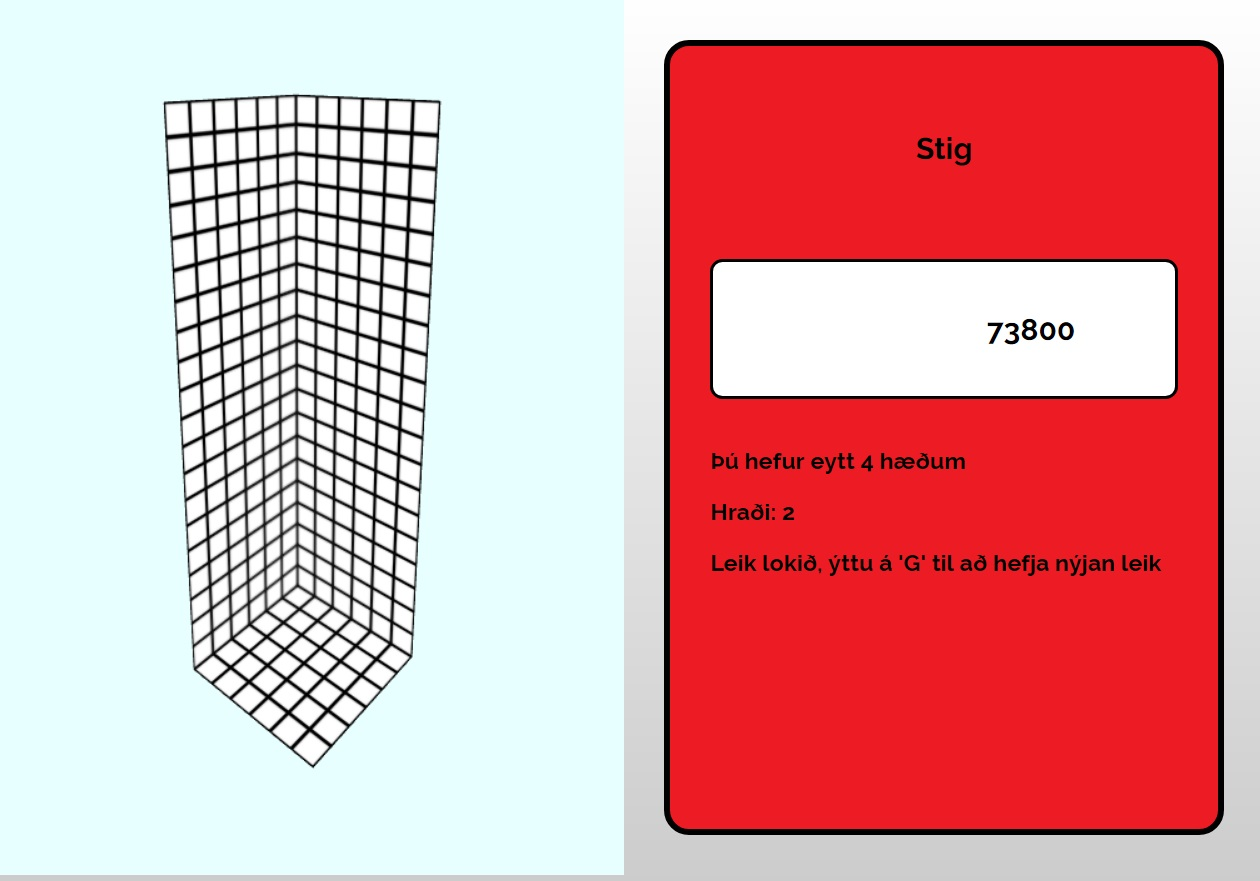
\includegraphics[scale=0.4]{m8}
\end{center}
Það ætti ekki að vera hægt að snúa kubbum út fyrir leiksvæðið eða snúa fallandi kubb inn í gamlan kubb, þess í stað helst kubburinn bara í sömu stöðu en hann hoppar ekki til.\\

Leikinn má spila á slóðinni:
\url{https://notendur.hi.is/~jgs7/tolvugrafik/Verkefni%203/kubbar.html}


\end{small}
\end{document}
